Ambas, materia oscura y energía oscura se detectan por sus efectos gravitacionales ya que una partícula de materia oscura aún no ha sido identificada, sin embargo, los nuevos experimentos y desarrollos tecnológicos han permitido alcanzar una sensibilidad tal que hace pensar en un descubrimiento inminente. A continuación expondremos algunas investigaciones que involucran a tales partículas que se realizan tanto en el espacio exterior, como en los laboratorios en la tierra.

\subsubsection{Rotación de las galaxias}
En la primera mitad del siglo pasado Paul Zwicky había estado observado agrupaciones de galaxias ligadas por atracción gravitatoria, siendo el primero en utilizar el \href{https://es.wikipedia.org/wiki/Teorema_del_virial}{Teorema de virial}, del estudio de las velocidades radiales de ocho galaxias en el cúmulo Coma, Zwicky encontró una dispersión de velocidad inesperadamente grande $\sigma_{cz} = (1019 \pm 360) ~ km ~ s^{-1}$ (recalculado en la actualidad por valor moderno $\sigma_{cz} = 1082 ~ km ~ s^{-1}$ obtenido por \cite{colless_structure_1996}). Zwicky concluyó de estas observaciones que la densidad media del grupo Coma tendría que ser $\backsim 400$ (valor moderno recalculado de $\backsim 50$) veces mayor que la derivada de la materia luminosa (se sobreestimó la relación masa-luz del grupo Coma por asumir un parámetro de Hubble de $H_o = 558 ~ km ~ s^{-1} ~Mpc^{-1}$ cuando su valor moderno de $H_o = 67.15~km~s^{-1} ~Mpc^{-1}$). Zwicky postula:

\begin{minipage}{0.9\linewidth}
\vspace{5pt}%margen superior de minipage
{\small }
\textit{``Si se confirma esta sobredensidad, llegaríamos a la sorprendente conclusión de que la materia oscura está presente en Coma con una densidad mucho mayor que la materia luminosa ... De estas consideraciones se deduce que la gran dispersión de velocidad en Coma representa un problema no resuelto''}
\begin{flushright}
presente en la referencia \cite{bergh_early_1999}
%(\citeauthor{Coulouris}, \citeyearNP{Coulouris}: 10)
\end{flushright}
\vspace{5pt}%margen inferior de la minipage
\end{minipage}

%\begin{figure}
%\centering
%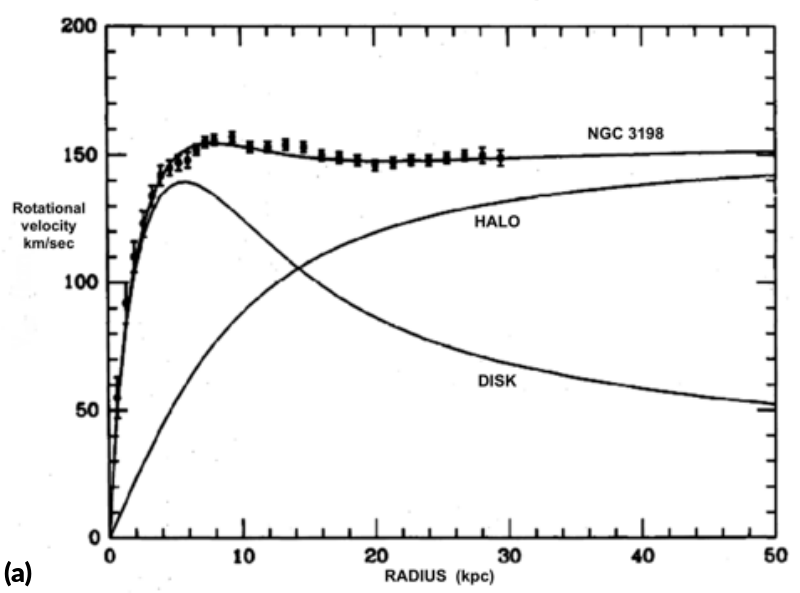
\includegraphics[width=0.49\textwidth]{Fisica_de_Particulas/imagenes/fritz.png}
%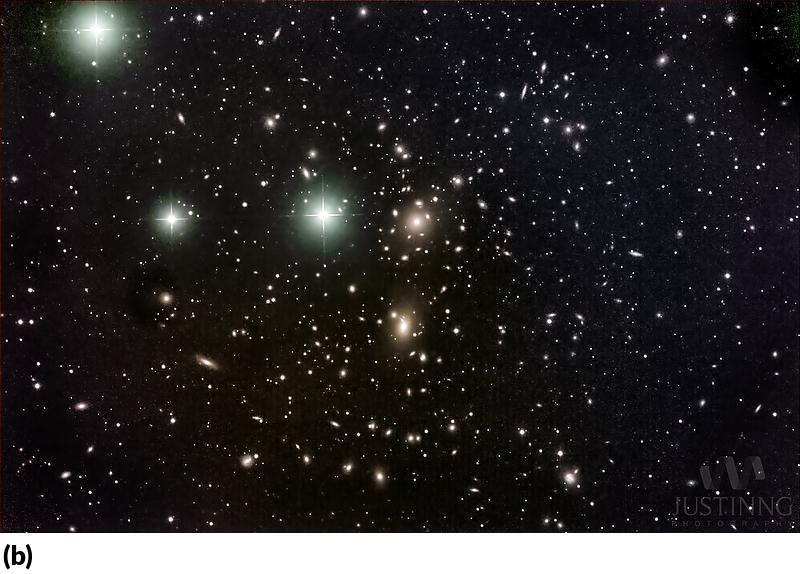
\includegraphics[width=0.49\textwidth]{Fisica_de_Particulas/imagenes/Coma-Cluster.jpg}
%\caption{(a) Gráficos de velocidad de rotación en función de la lejania del centro de la galaxia NGC 3198. Página de origen: \url{https://earthsky.org/clusters-nebulae-galaxies/the-coma-berenices-galaxy-cluster}, (b) Visualización del cúmulo de $\backsim 10^4$ galaxias Coma. Página de origen: \url{https://earthsky.org/clusters-nebulae-galaxies/the-coma-berenices-galaxy-cluster}}
%\label{coma}
%\end{figure}
%Esta cuestión continuo siendo un enigma hasta que Vera Rubin y Kent Ford confirmaron la prueba de su existencia en 1970 al trazar la curva de rotación de la galaxia ver el gráfico correspondiente a la Fig. \ref{coma}a para \href{https://en.wikipedia.org/wiki/NGC_3198}{NGC 3198} (es una galaxia espiral en la constelación de la Osa Mayor) muestra que la velocidad de la materia visible es esencialmente constante aunque nos elejemos del centro para distancias mayores de $\gtrsim 5 ~kpc$ desde el centro de la galaxia, en lugar de tener una caída Kepleriana proporcional a $1/r$. 

En la actualidad se continuan los intentos por comprender el problema galáctico de la masa visible faltante, ejemplos se pueden encontrar proyectos de simulaciones \citep{deur_relativistic_2020, wu_galactic_2015} o mediante la comparacion empírica con los datos experimentales \cite{mielke_dark_2006}, con altos niveles de predicción.


\subsubsection{Lentes gravitacionales}
Otra evidencia viene de las \href{https://en.wikipedia.org/wiki/Gravitational_lens}{lentes gravitacionales} (Fig. \ref{lentes}). La gravedad afecta a todo el espectro de ondas electromagnéticas, incluyendo radio, infrarrojos, luz visible y ultravioleta, siendo el grado de desviación mayor mientras mayor sea la masa que actúa como lente gravitacional, siento esta predicción unos de los mayores resultados de Einstein, en estos cálculos se pudo evidenciar el efecto para cálcular el valor de masas de grandes cúmulos midiendo las desviaciones de la luz.

\begin{figure}[h]
\centering
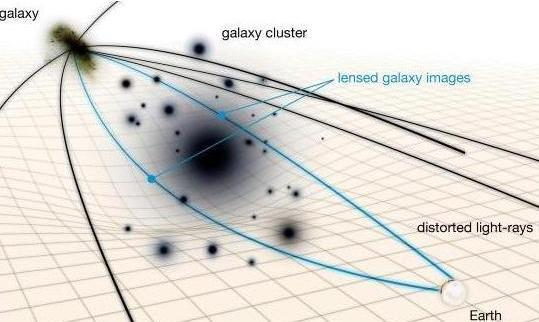
\includegraphics[width=.6\textwidth]{Fisica_de_Particulas/imagenes/lentes.jpg}
\caption{Diagrama de cúmulo de galaxias que actúa como lente gravitatoria para una galaxia muy distante. %El efecto de la masa es el de curvar el espacio-tiempo, alterando las trayectorias de la luz que emite la galaxia.
Página de origen: \url{https://alquimiayciencias.blogspot.com/2013/06/explicando-la-materia-oscura-cualquiera.html}%, (b) Imagen del cúmulo de galaxias Abell 3827 obtenida por el Telescopio Espacial Hubble. Página de origen: \url{https://astronomy.com/news/2015/04/dark-matter-may-not-be-completely-dark-after-all} %https://vaticanobservatory.wordpress.com/2015/04/21/imagem-hubble-do-aglomerado-de-galaxias-abell-3827-que-mostra-a-distribuicao-da-materia-escura/}
}
\label{lentes}
\end{figure}
Dadas sus características los \href{https://curiosoando.com/introduccion-a-las-lentes-gravitacionales}{lentes gravitacionales} son un importante herramienta para detectar la materia oscura, resultado de la comparación de lo resultados experimentales con los resultados de la relatividad general que predice la dinámica dependiente de la masa visible. 

%En algunos casos, la lente no es lo suficientemente fuerte como para formar múltiples imágenes o arcos, sin embargo, la fuente aún está distorsionada porque es un hecho que hay algo de materia oscura entre nosotros y cada galaxia distante que vemos, %de aca que todas las galaxias tienen lentes, incluso si son solo un poco, 
%aquellas alteradas solo en una cantidad muy pequeña son llamadas lentes gravitacionales débiles.
%\begin{figure}[h]
%\centering
%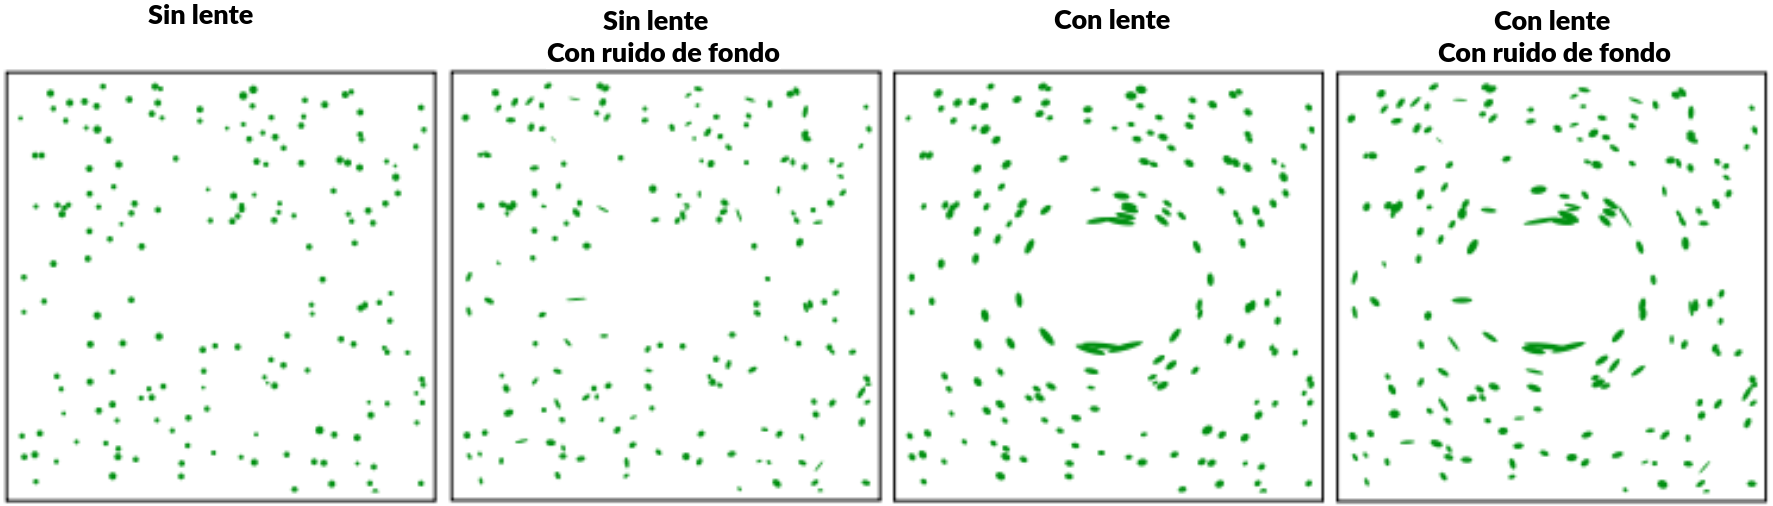
\includegraphics[width=1\textwidth]{Fisica_de_Particulas/imagenes/lentes.png}
%\caption{Simulación de un campo de galaxias circulares, el ruido de fondo es un grupo de galaxias realista de fondo. Página de origen: \url{https://fos.cmb.ac.lk/blog/gravitational-lensing-wonders-universe-iii/}}
%\label{lentes2}
%\end{figure}
%Nunca podemos ver esta modificación de forma con nuestros propios ojos en una imagen porque es demasiado pequeña, en vez de eso podemos calcular el efecto de lente promedio en un conjunto de galaxias, normalmente bajo suposiciones (ver Fig. \ref{lentes2}), como considerar que todas las galaxias tienen una formas elípticas o que están orientadas al azar en el cielo, estas se traten de forma estadística.

%Trabajos dedicados a la simulación numérica (ver referencia \citep{munshi_statistics_2001, fosalba_mice_2015}) para conocer los efectos de la distribución de la materia oscura en un el universo (ver Fig. \ref{lentes3}), las trayectorias de los rayos se desvían evidentemente por los efectos gravitacionales de la materia provocando que las galaxias esten ligeramente alargadas en una dirección común determinada por la distribución de la materia oscura a lo largo de esa línea de visión particular, ya que la distorsión es muy pequeña, esta requiere un tratamiento estadístico cuidadoso en muchos parches en el cielo.
%\begin{figure}[h]
%\centering
%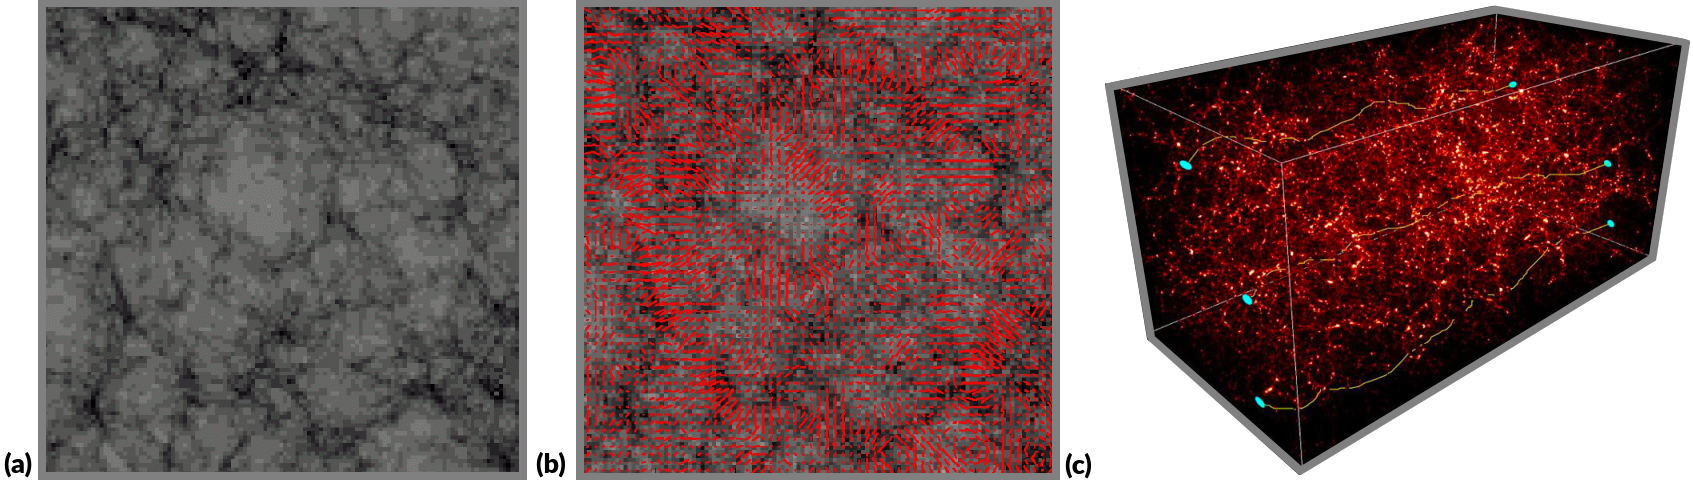
\includegraphics[width=1\textwidth]{Fisica_de_Particulas/imagenes/lentes3.png}
%\caption{(a) Simulación computacional de materia oscura, (b) Efecto lente gravitación, (c) Simulación numérica que muestra la distribución de la materia oscura en un gran volumen del universo,  los tres discos azules representan tres galaxias distantes, Las líneas que cruzan la caja representan rayos de luz de esas galaxias que se propagan a través del universo. Página de origen: \url{http://www.cfht.hawaii.edu/News/Lensing/index.html\#ST}}
%\label{lentes3}
%\end{figure}
%Las lentes gravitacionales fuertes se caracterizan por la curvada distorsión observada de las galaxias de fondo, estas han sido observada alrededor de un cúmulo poco distante como el Abell 1689 o 3827. %(ver Fig. \ref{lentes}b). Midiendo la distorsión geométrica, se puede obtener la masa del cúmulo que causa el fenómeno. Estas lentes permiten ver objetos distantes, sobre todo galaxias lejanas, al intensificar su luz, motivo por el cual su estudio es motivo de investigación (\cite{schafer_lenstool-hpc_2020}). Al observar la luz de las galaxias más distantes, algunas tan antiguas que su formación se remonta a las primeras fases de expansión del Universo, los astrónomos pueden estudiar las condiciones de hace miles de millones de años, e incluso que sucedía durante la formación de estas galaxias, de forma que pueden ser aplicadas de modo similar a los telescopios. Un caso especial de estos lentes son los \href{https://en.wikipedia.org/wiki/Einstein_ring}{anillos de Einstein}, causada por la alineación exacta de la fuente, la lente y el observador, este fue predicho por este en 1912.

%Las microlentes se suelen formar por el paso de una estrella o planeta delante de otra estrella u otro objeto más lejano. La luz del objeto distante no está tan distorsionada como en las lentes fuertes, ni siquiera alcanza a la distorsión de las lentes débiles; la distorsión de la imagen puede ser prácticamente imperceptible, pero la disminución en la intensidad de la luz pone de manifiesto las microlentes. Gracias a las microlentes se han descubierto numerosos planetas extrasolares.

\subsubsection{Coalisión de galaxias}
\begin{figure}[h]
\centering
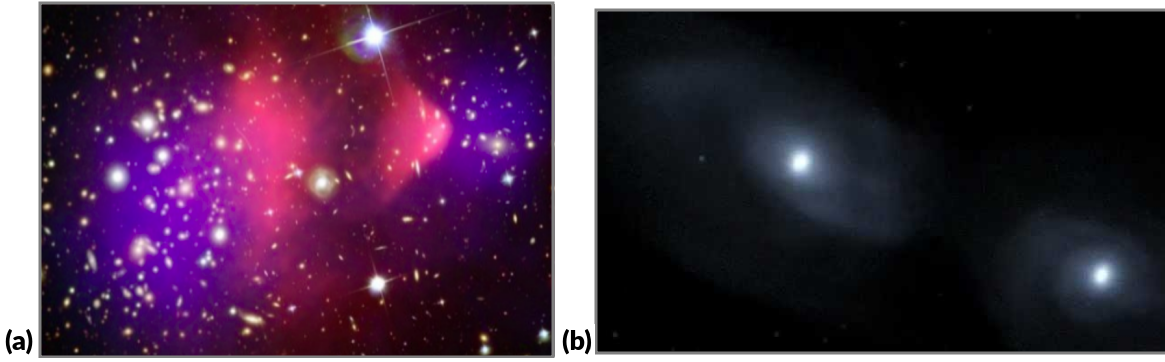
\includegraphics[width=.7\textwidth]{Fisica_de_Particulas/imagenes/fritz2.png}
\caption{
(a) Coalisión de dos cúmulos de galaxias 1E 0657-56 conocida como \href{https://en.wikipedia.org/wiki/Bullet_Cluster}{cúmulo bala}. %Página de origen: \url{https://en.wikipedia.org/wiki/Bullet_Cluster\#/media/File:1e0657_scale.jpg} 
, (b) Simulación por computadora de la futura colisión prevista de las dos galaxias más grandes del Grupo Local, Andrómeda (M31) y la Vía Láctea. %Página de origen: \url{https://hubblesite.org/contents/media/videos/2012/20/700-Video.html?news=true} 
}
\label{coalision}
\end{figure}
Los científicos usaron el observatorio Chandra de rayos X de la NASA y el Telescopio Espacial Hubble para estudiar el grupo, conocido como MACSJ0025.4-1222, donde se enfoca una colisión de dos cúmulos de galaxias (ver Fig. \ref{coalision}a)%, en esta las dos áreas rosadas contienen la mayor parte de la masa ordinaria de los dos grupos, el uno en forma de bala pasó a través del otro grupo más grande
. 

En el proceso de la colisión, la temperatura de la materia normal aumenta y se emiten rayos X que fueron detectados por el Observatorio de Rayos X Chandra. Las áreas azules son un mapa de la materia invisible hecha mediante el uso de lentes gravitacionales, donde la luz de los objetos más distantes que el grupo de balas se dobla por la materia que interviene. La materia normal que se muestra en rosa está claramente separada de la mayoría de la materia que comprende los grupos que se muestran en azul. La conclusión es que la mayor parte de la materia en los grupos es materia oscura\cite{marsh_strings_2019}.

%Dada la riqueza en el fenómeno de coalisión este es ampliamente estudiado incluso en la actualidad en el 2018 la \textbf{UNAM} (Universidad Nacional Autónoma de México) diseñó el \textbf{NEFER} (Nuevo Espectrómetro Fabry-Perot de Extrema Resolución), invento integrable al espectrómetro \textbf{OSIRIS} del Gran Telescopio Canarias (GTC) en España, permitiendo observar en dos dimensiones de alta resolución la formación estelar que se produce en las galaxias e inclusive la distribución de la materia oscura, todo mediente mapas bidimensionales de intensidades y velocidades de objetos astronómicos extendidos, diseñado principalmente para observar la emisión y las velocidades del medio interestelar de nuestra galaxia y de galaxias externas.

%La complejidad de estos fenómenos esta siendo arduamente estudiada, bajo la apuesta de que nuestra comprensión del mundo mejorara por ello, razón por lo cual los trabajos en esa linea son tema actual implementando continuamente la simulación como herramienta de análisis, este fue el caso de dos galaxias Andrómeda (M31) y la Vía Láctea, las cuales formaron parte de un arduo trabajo basada su predicción en mediciones con el telescopio espacial Hubble del movimiento adecuado de M31 en el cielo, junto con el desplazamiento al rojo de M31 (ver Fig. \ref{coalision})c relacionado con la referencia \cite{van_der_marel_m31_2012}. 
%Mientras previas investigaciones afirman la necesidad de incluir la materia oscura en las simulaciones hay que considerar algunas investigaciones que bajo el excepticismo de la existencia de materia oscura intenta encontrar otras fuentes de incertidumbre, posibles soluciones como sos presentados en la referencia \cite{bilek_mond_2018}, donde se intentan adaptar la relatividad general bajo un nuevo enfoque dada por la teoría \href{https://en.wikipedia.org/wiki/Modified_Newtonian_dynamics}{\textbf{MOND}} (del inglés \href{https://en.wikipedia.org/wiki/Modified_Newtonian_dynamics}{Modified Newtonian dynamics}) dando resultados que hacen cuestionar que tan cerca estamos de entender la materia oscura o su existencia.


\subsubsection{Formación de estructuras}

%En las simulaciones la inclusión de la materia oscura es fundamental para explicar la formación de estructuras cosmologicas ya que la materia normal sucumbe a la fuerza de atracción de la materia oscura formando galaxias y cúmulos de ellas, por otro lado la energía oscura es cualquier entidad que haga que la expansión del universo se acelere.

La historia del universo es la competencia entre la materia oscura que lo frena y la energía oscura que lo acelera. A medida que el espacio se expande, la materia y la radiación se diluyen; en cambio, la densidad del vacío permanece constante, y por eso triunfará en la competencia, el universo se expandirá cada vez a un ritmo mayor y esa aceleración tiene importantísimas consecuencias para el futuro del universo, de aquí que sea crucial para el modelo cosmológico del Big Bang como un componente que se corresponde directamente con las medidas de los parámetros asociados con la métrica \href{https://es.wikipedia.org/wiki/M\%C3\%A9trica_de_Friedman-Lema\%C3\%AEtre-Robertson-Walker}{\textbf{FLRW}} (métrica de Friedmann-Lemaître-Robertson-Walker) a la relatividad general. 

%Las anisotropías del \CMB ~ se corresponden a una cosmología donde gran parte de la materia interactúa con los fotones de forma más débil que las fuerzas fundamentales conocidas que acoplan las interacciones de la luz con la materia bariónica. Así mismo, se necesita una cantidad significativa de materia fría no-barionica para explicar la estructura a gran escala del universo. %Las observaciones sugieren que la formación de estructuras en el Universo procede jerárquicamente, con las estructuras más pequeñas uniéndose hasta formar galaxias y después cúmulos de galaxias. 
Según se unen las estructuras en la evolución del Universo, empiezan a "brillar" ya que la materia bariónca se calienta a través de la contracción gravitacional y los objetos se aproximan al equilibrio hidrostático. La materia barionica ordinaria tendría una temperatura demasiado alta y demasiada presión liberada desde el Big Bang para colapsar y formar estructuras más pequeñas, como estrellas, a través de la inestabilidad de Jeans. La materia oscura actúa como un compactador de estructuras. %Este modelo no sólo se corresponde con investigaciones estadísticas de la estructura visible en el Universo sino también se corresponden de forma precisa con las predicciones de materia oscura de la \WMAP.

%Para obtener el inverso de formación de estructuras necesita algún tipo de la materia oscura para funcionar. Se han utilizado simulaciones por ordenador de miles de millones de partículas de materia oscura para confirmar que el modelo de materia oscura fría de la formación de estructuras es consistente con las estructuras observadas en el Universo mediante las observaciones de galaxias, como la Sloan Digital Sky Survey y la 2dF Galaxy Redshift Survey, así como las observaciones del bosque Lyman-alfa. Estos estudios han sido cruciales en la construcción del modelo Lambda-CDM que mide los parámetros cosmológicos, incluyendo la parte del Universo formada por bariones y la materia oscura.













